
\documentclass[a4paper,12pt]{article}

\usepackage{graphicx}
\usepackage{a4wide}
\usepackage{lineno}
\usepackage{setspace}
  \doublespacing
\usepackage[document]{ragged2e}


\begin{document}
{\Large Comparison of large-scale citizen science data and long-term study data for phenology modeling \par}

\textit{Shawn D. Taylor, Joan M. Meiners, Kristina Riemer, Michael C. Orr, Ethan P. White}

\textbf{\large Supplementary materials}

Supplementary images S1 - S7 and Table S1

%%%%%%%%%%%%%%%%%
%% Figure S1
%%%%%%%%%%%%%%%%%
\newpage

\textbf{Figure S1}: RMSE for specific species and phenophases of the USA-NPN dataset. X marks the best performing models for each respective data type.

\newpage

\begin{center}
	\centering
		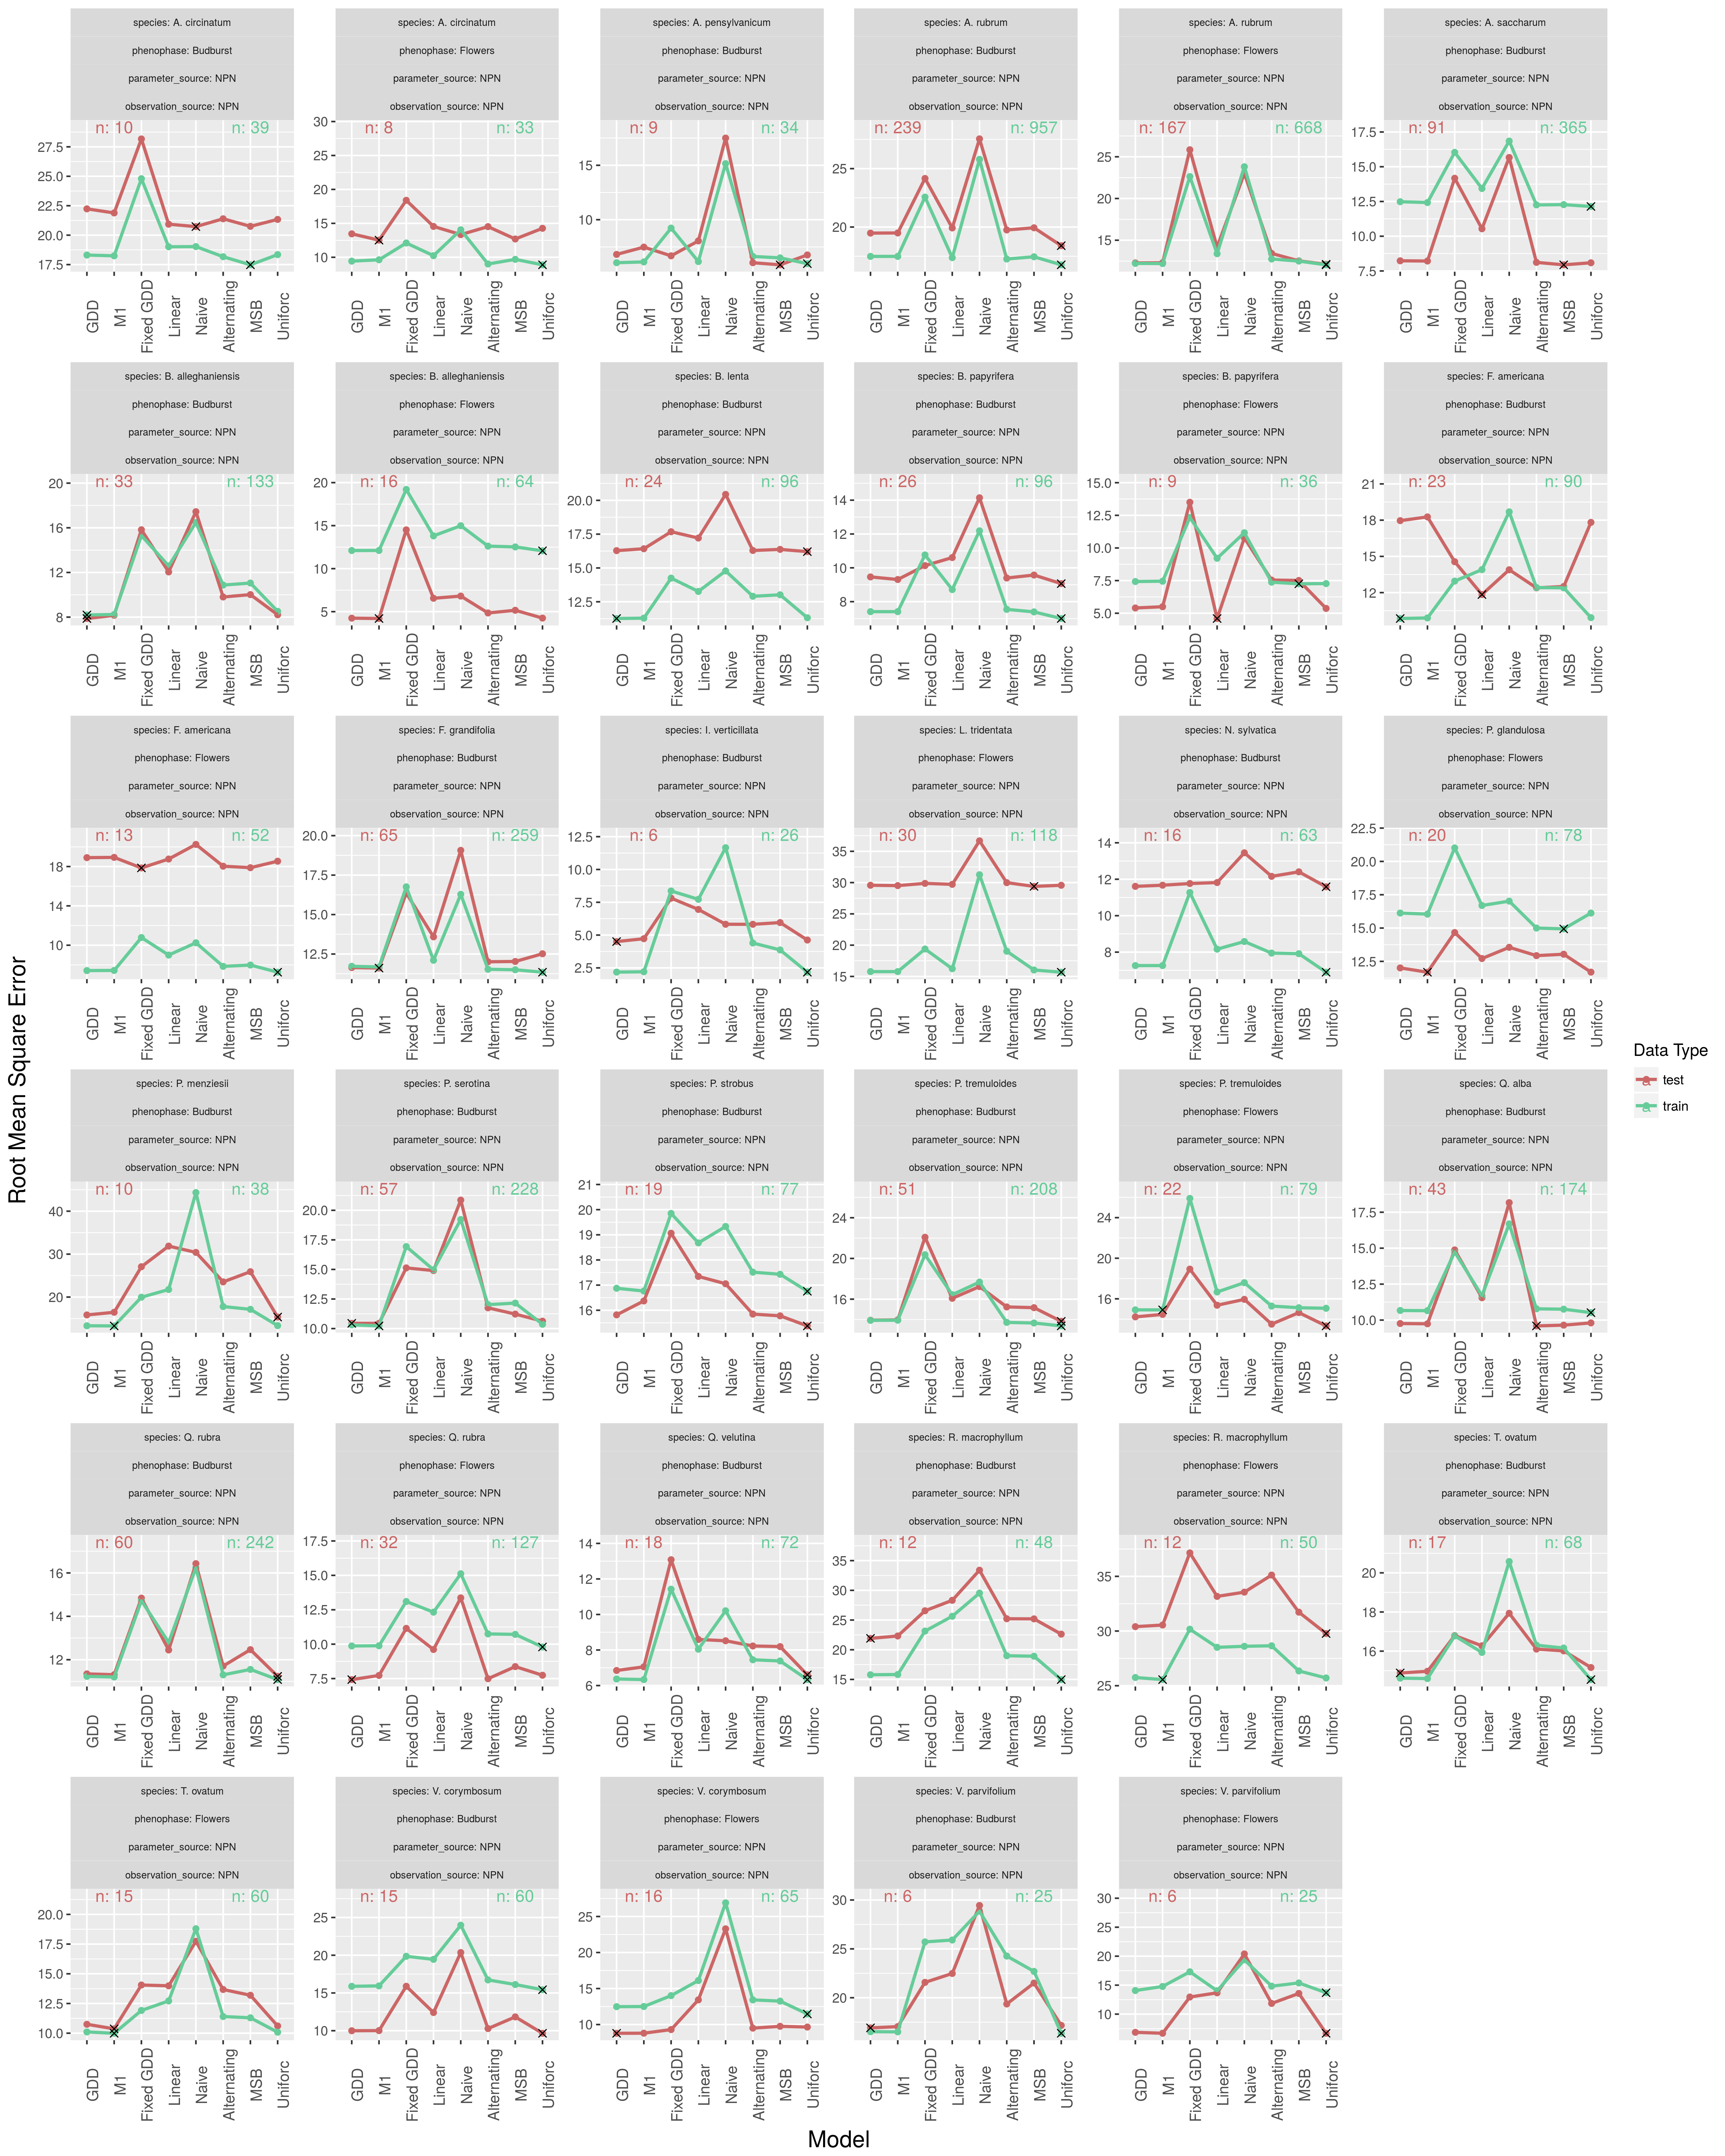
\includegraphics[width=1\textwidth]{supplement_best_npn_models.png}
	Figure S1
\end{center}

\newpage
%%%%%%%%%%%%%%%%%
%% Figure S2
%%%%%%%%%%%%%%%%%
\textbf{Figure S2}: RMSE for specific species and phenophases of the LTER datasets. X marks the best performing models for each respective data type.

\newpage

\begin{center}
	\centering
		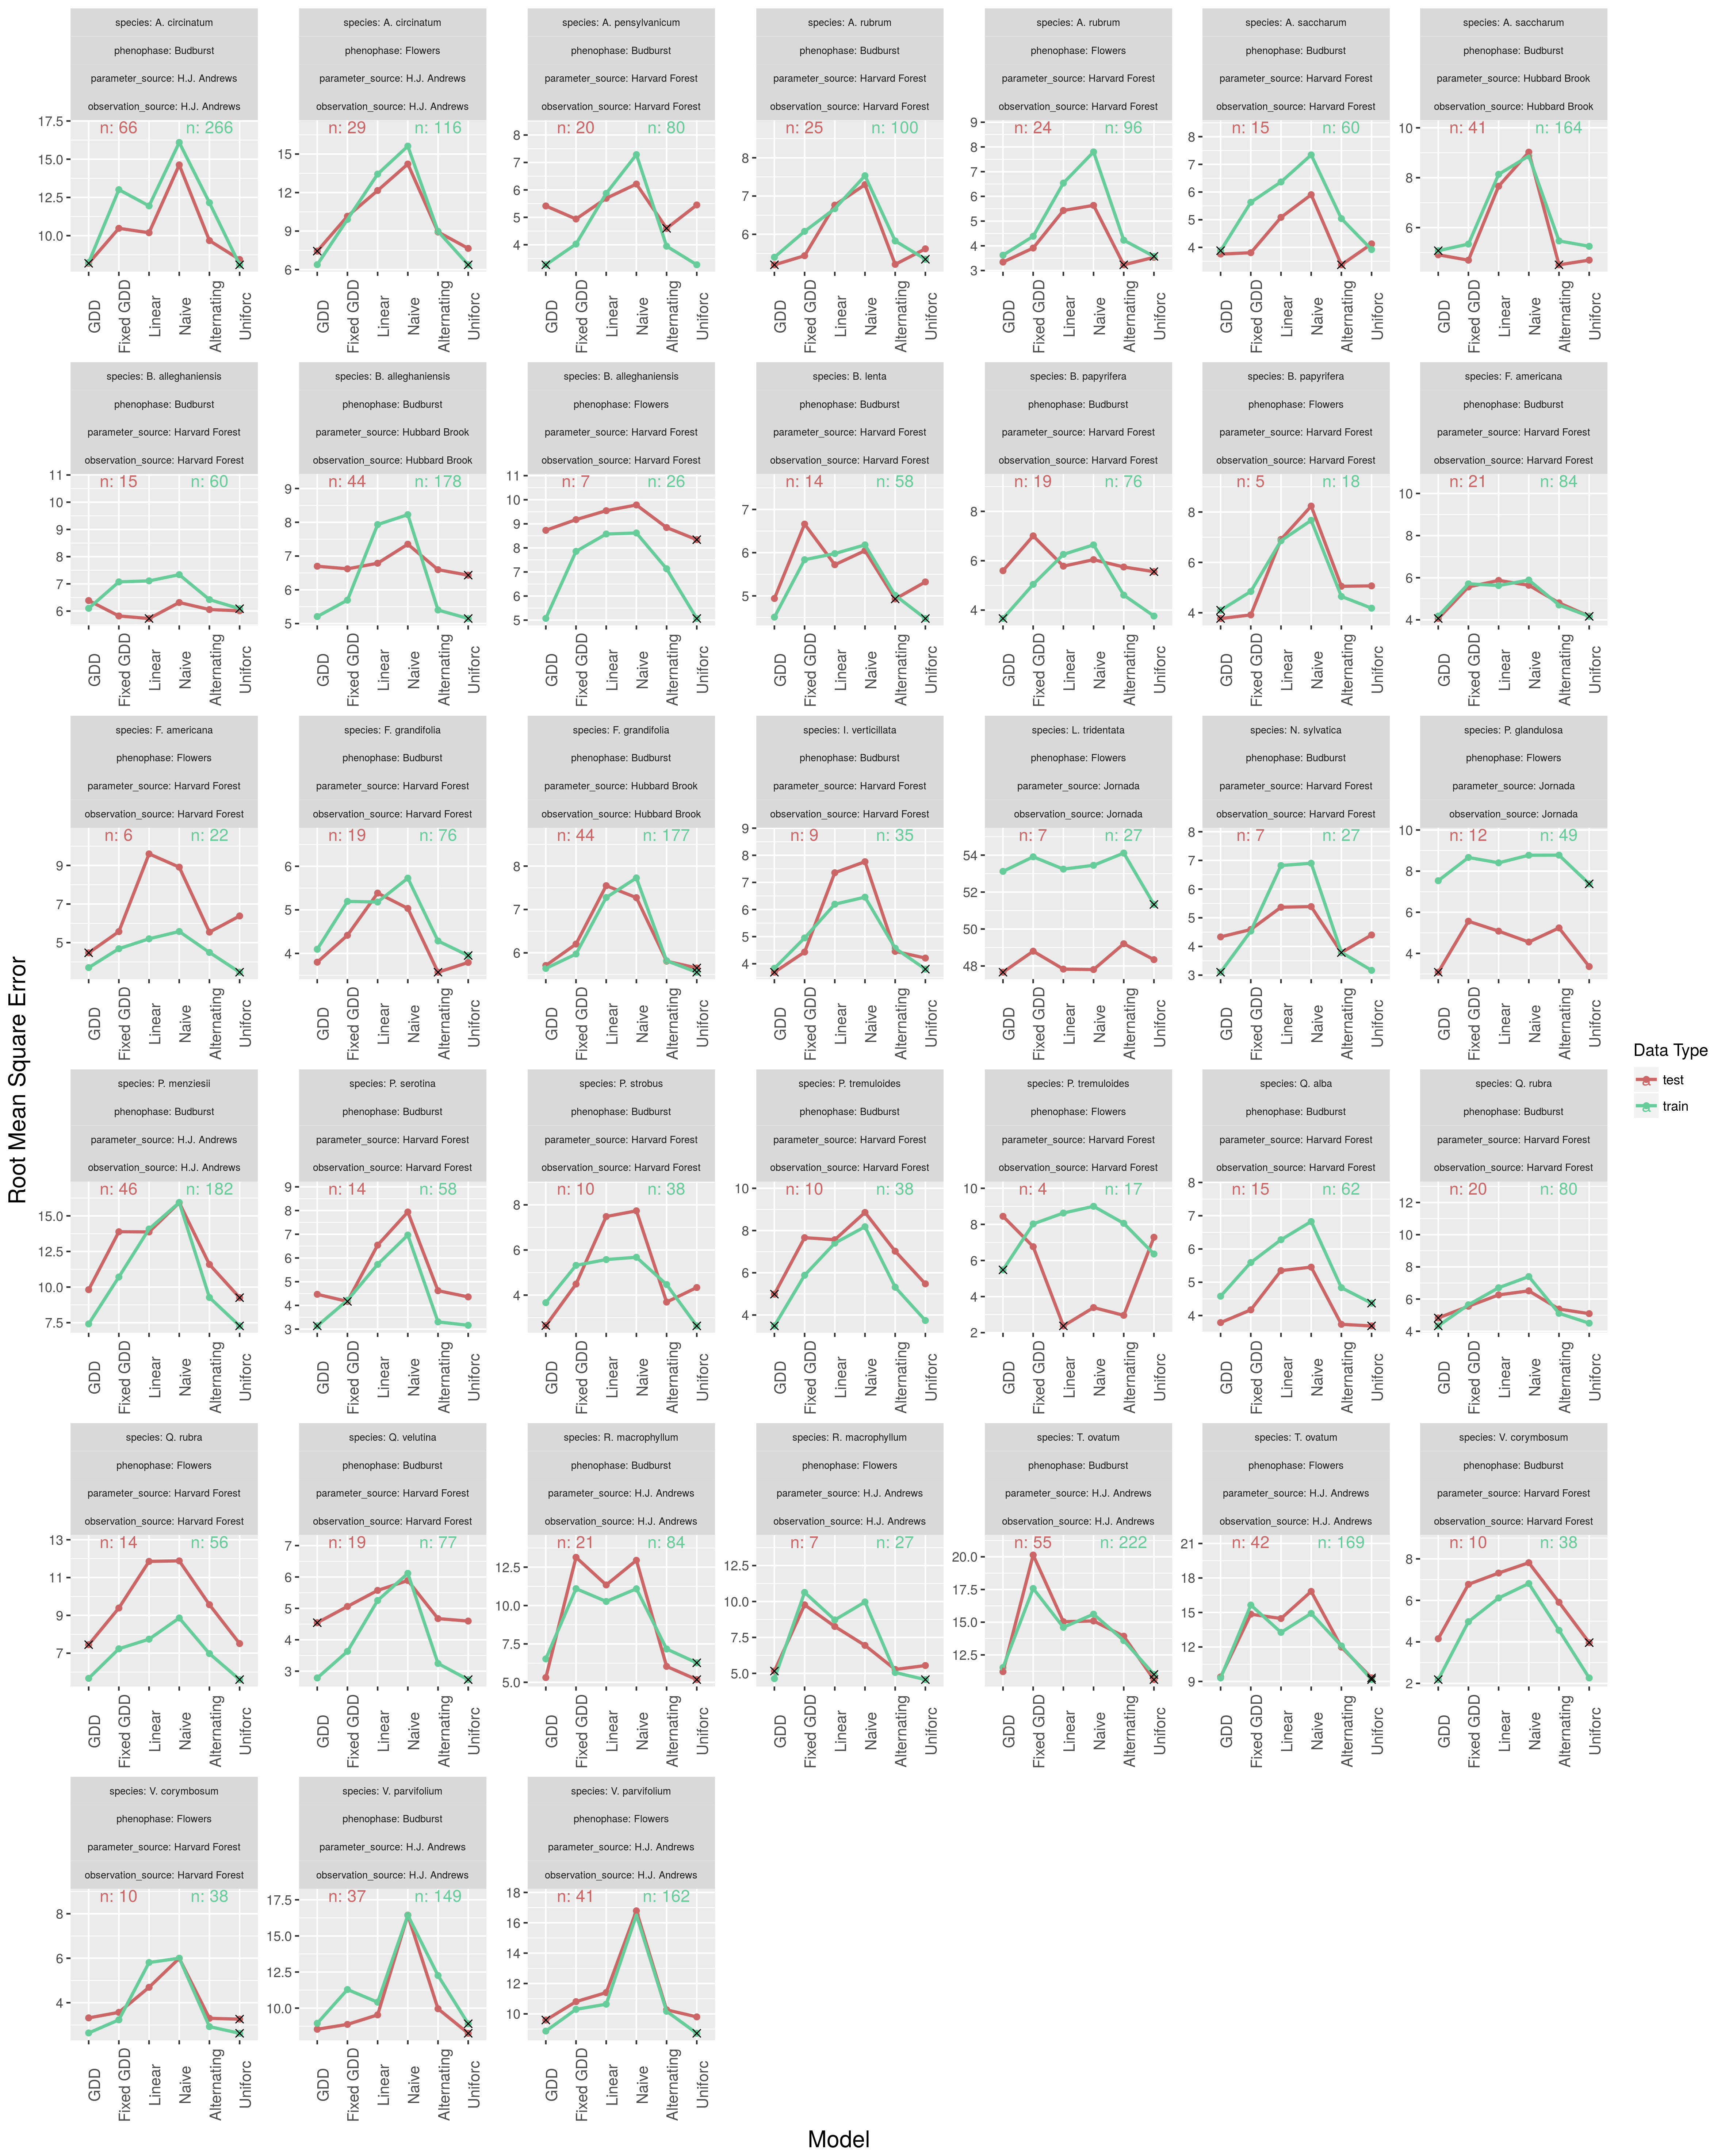
\includegraphics[width=1\textwidth]{supplement_best_lter_models.png}
	Figure S2
\end{center}

%%%%%%%%%%%%%%%%%
%% Figure S3
%%%%%%%%%%%%%%%%%

\newpage

\textbf{Figure S3}: RMSE of all species and phenophases of the four scenarios described in the text. These values were calculated using held out test data.

\newpage

\begin{center}
	\centering
		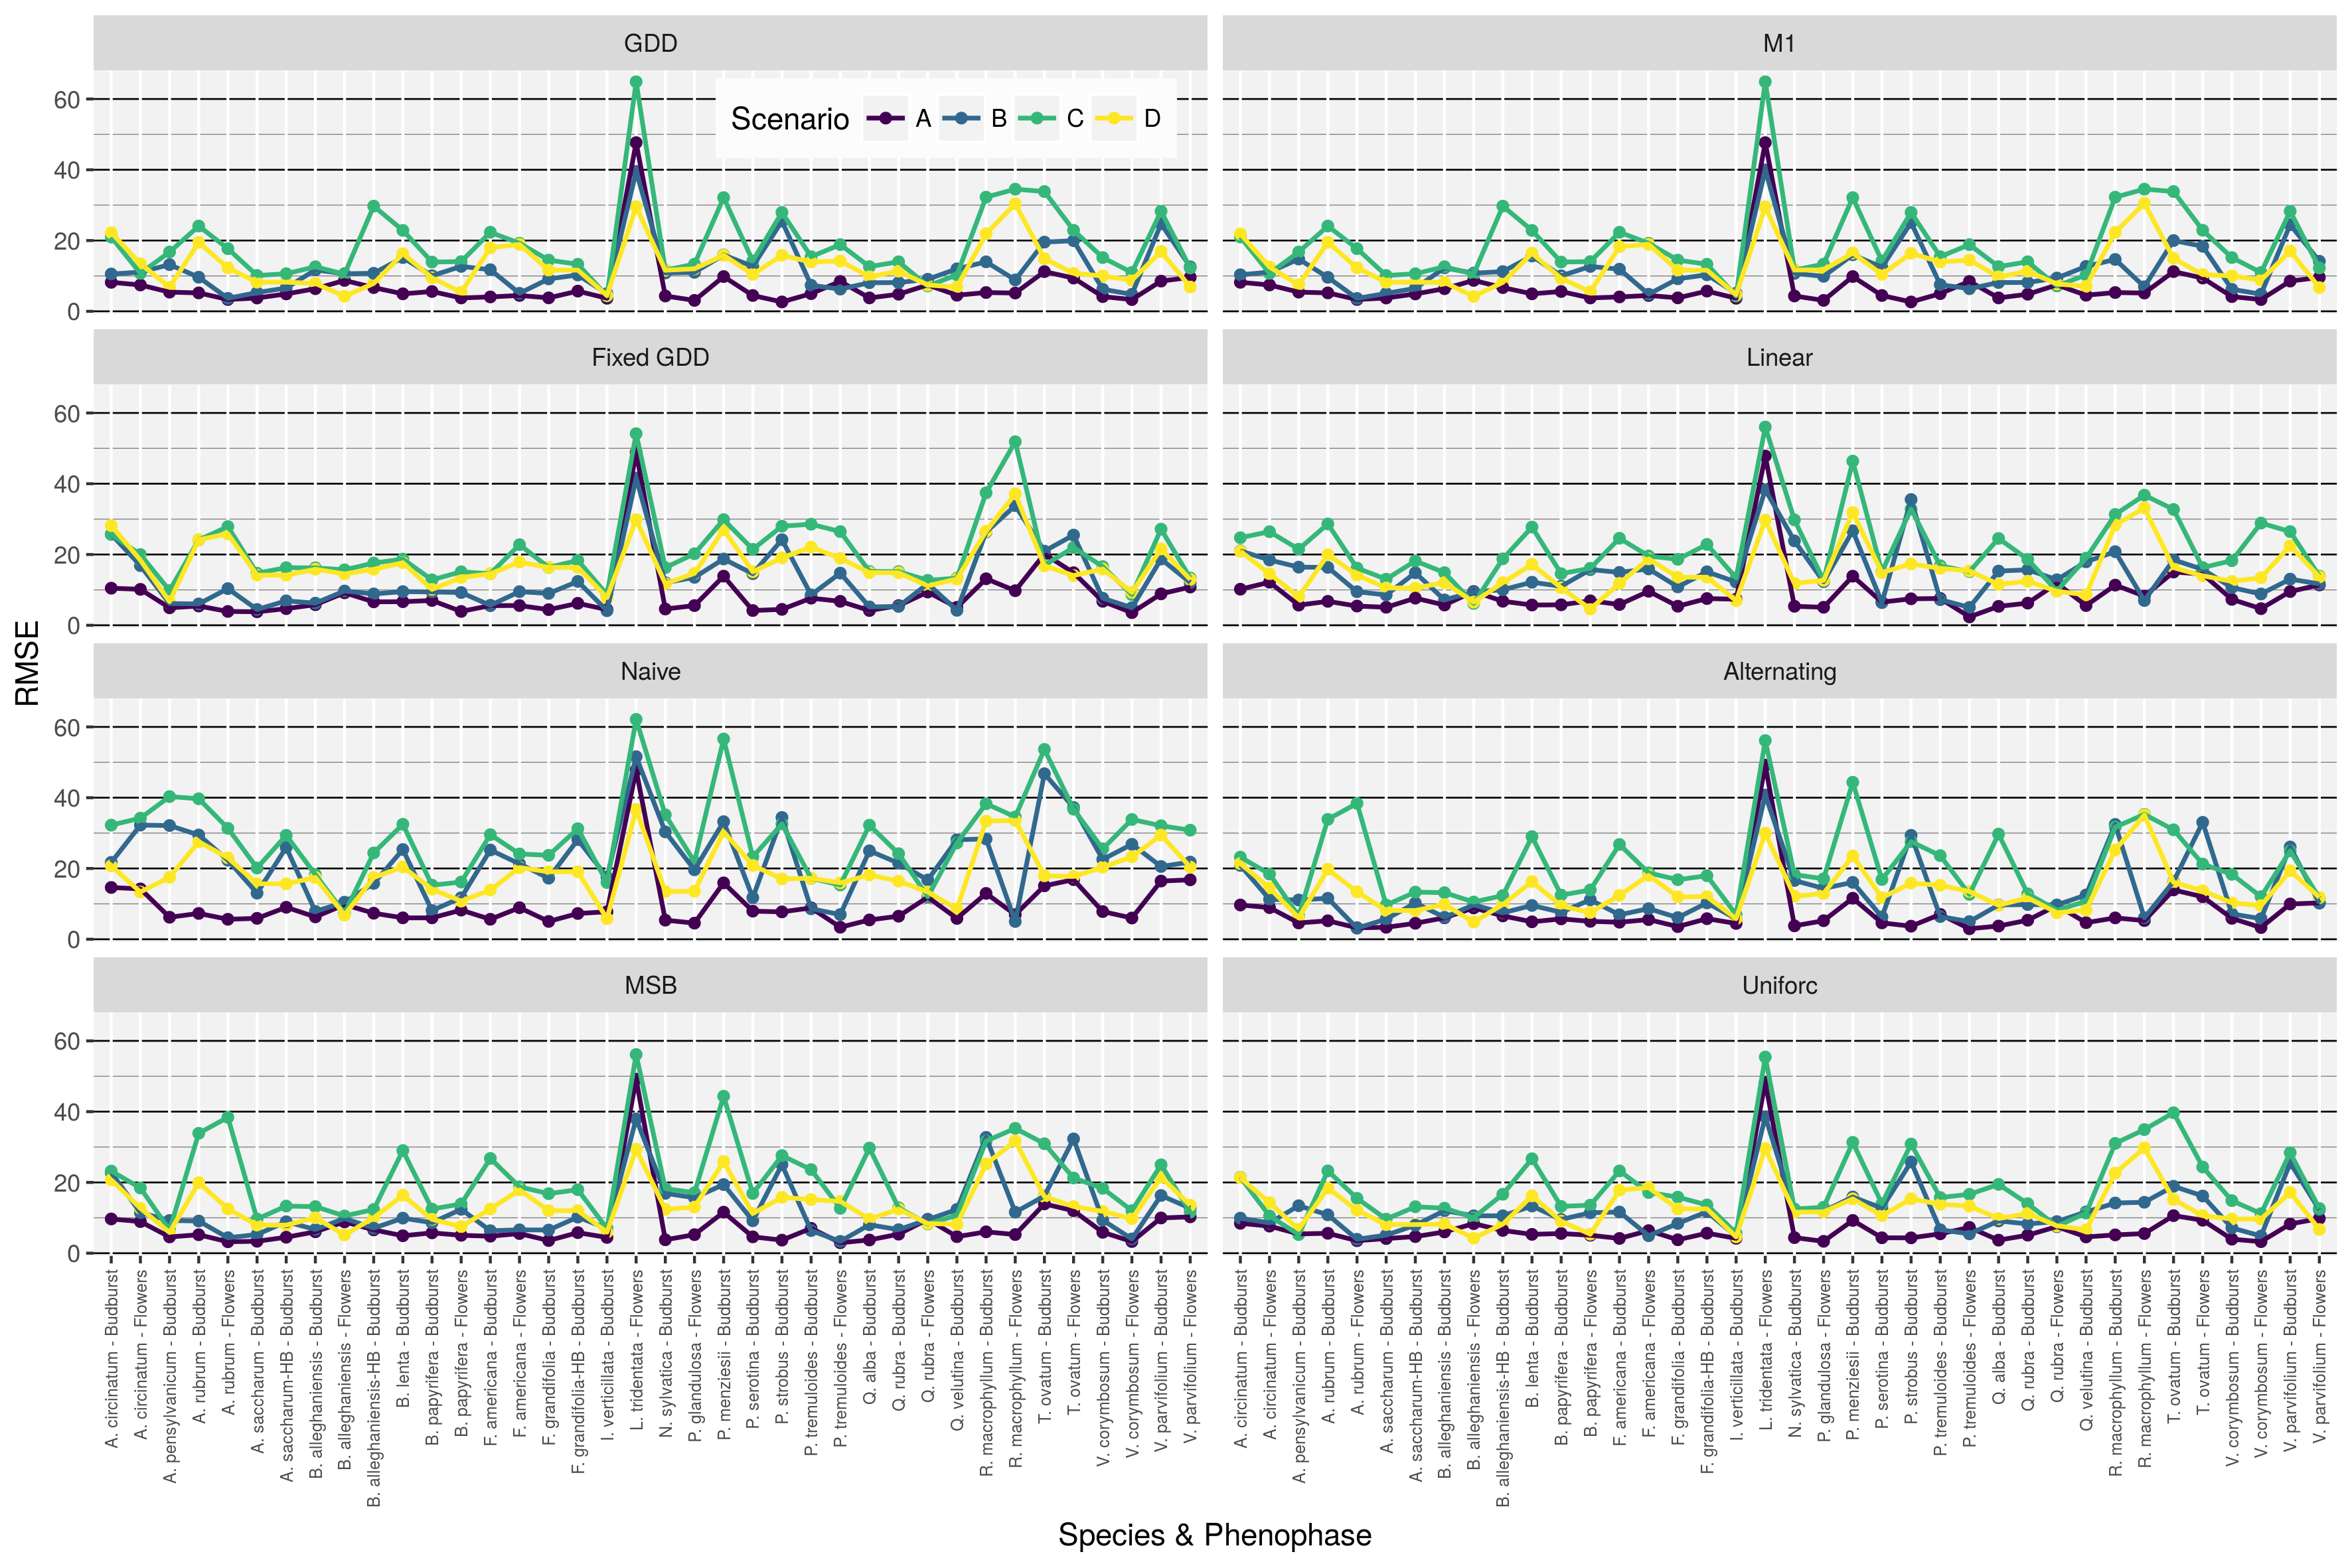
\includegraphics[width=1\textwidth]{supplement_scenario_absolute_rmse.png}
	Figure S3
\end{center}

%%%%%%%%%%%%%%%%%
%% Figure S4
%%%%%%%%%%%%%%%%%
\newpage

\textbf{Figure S4}: Distribution of parameters of the Naive, GDD, Fixed GDD, and Linear models for the three species common to the Hubbard Brook, Harvard, and USA-NPN datasets. The phenophase is budburst for all three species. Vertical lines indicate either the mean (solid) or median (dashed) of the respective distribution. Note the heading for each sub figure. 

\newpage

\begin{center}
	\centering
		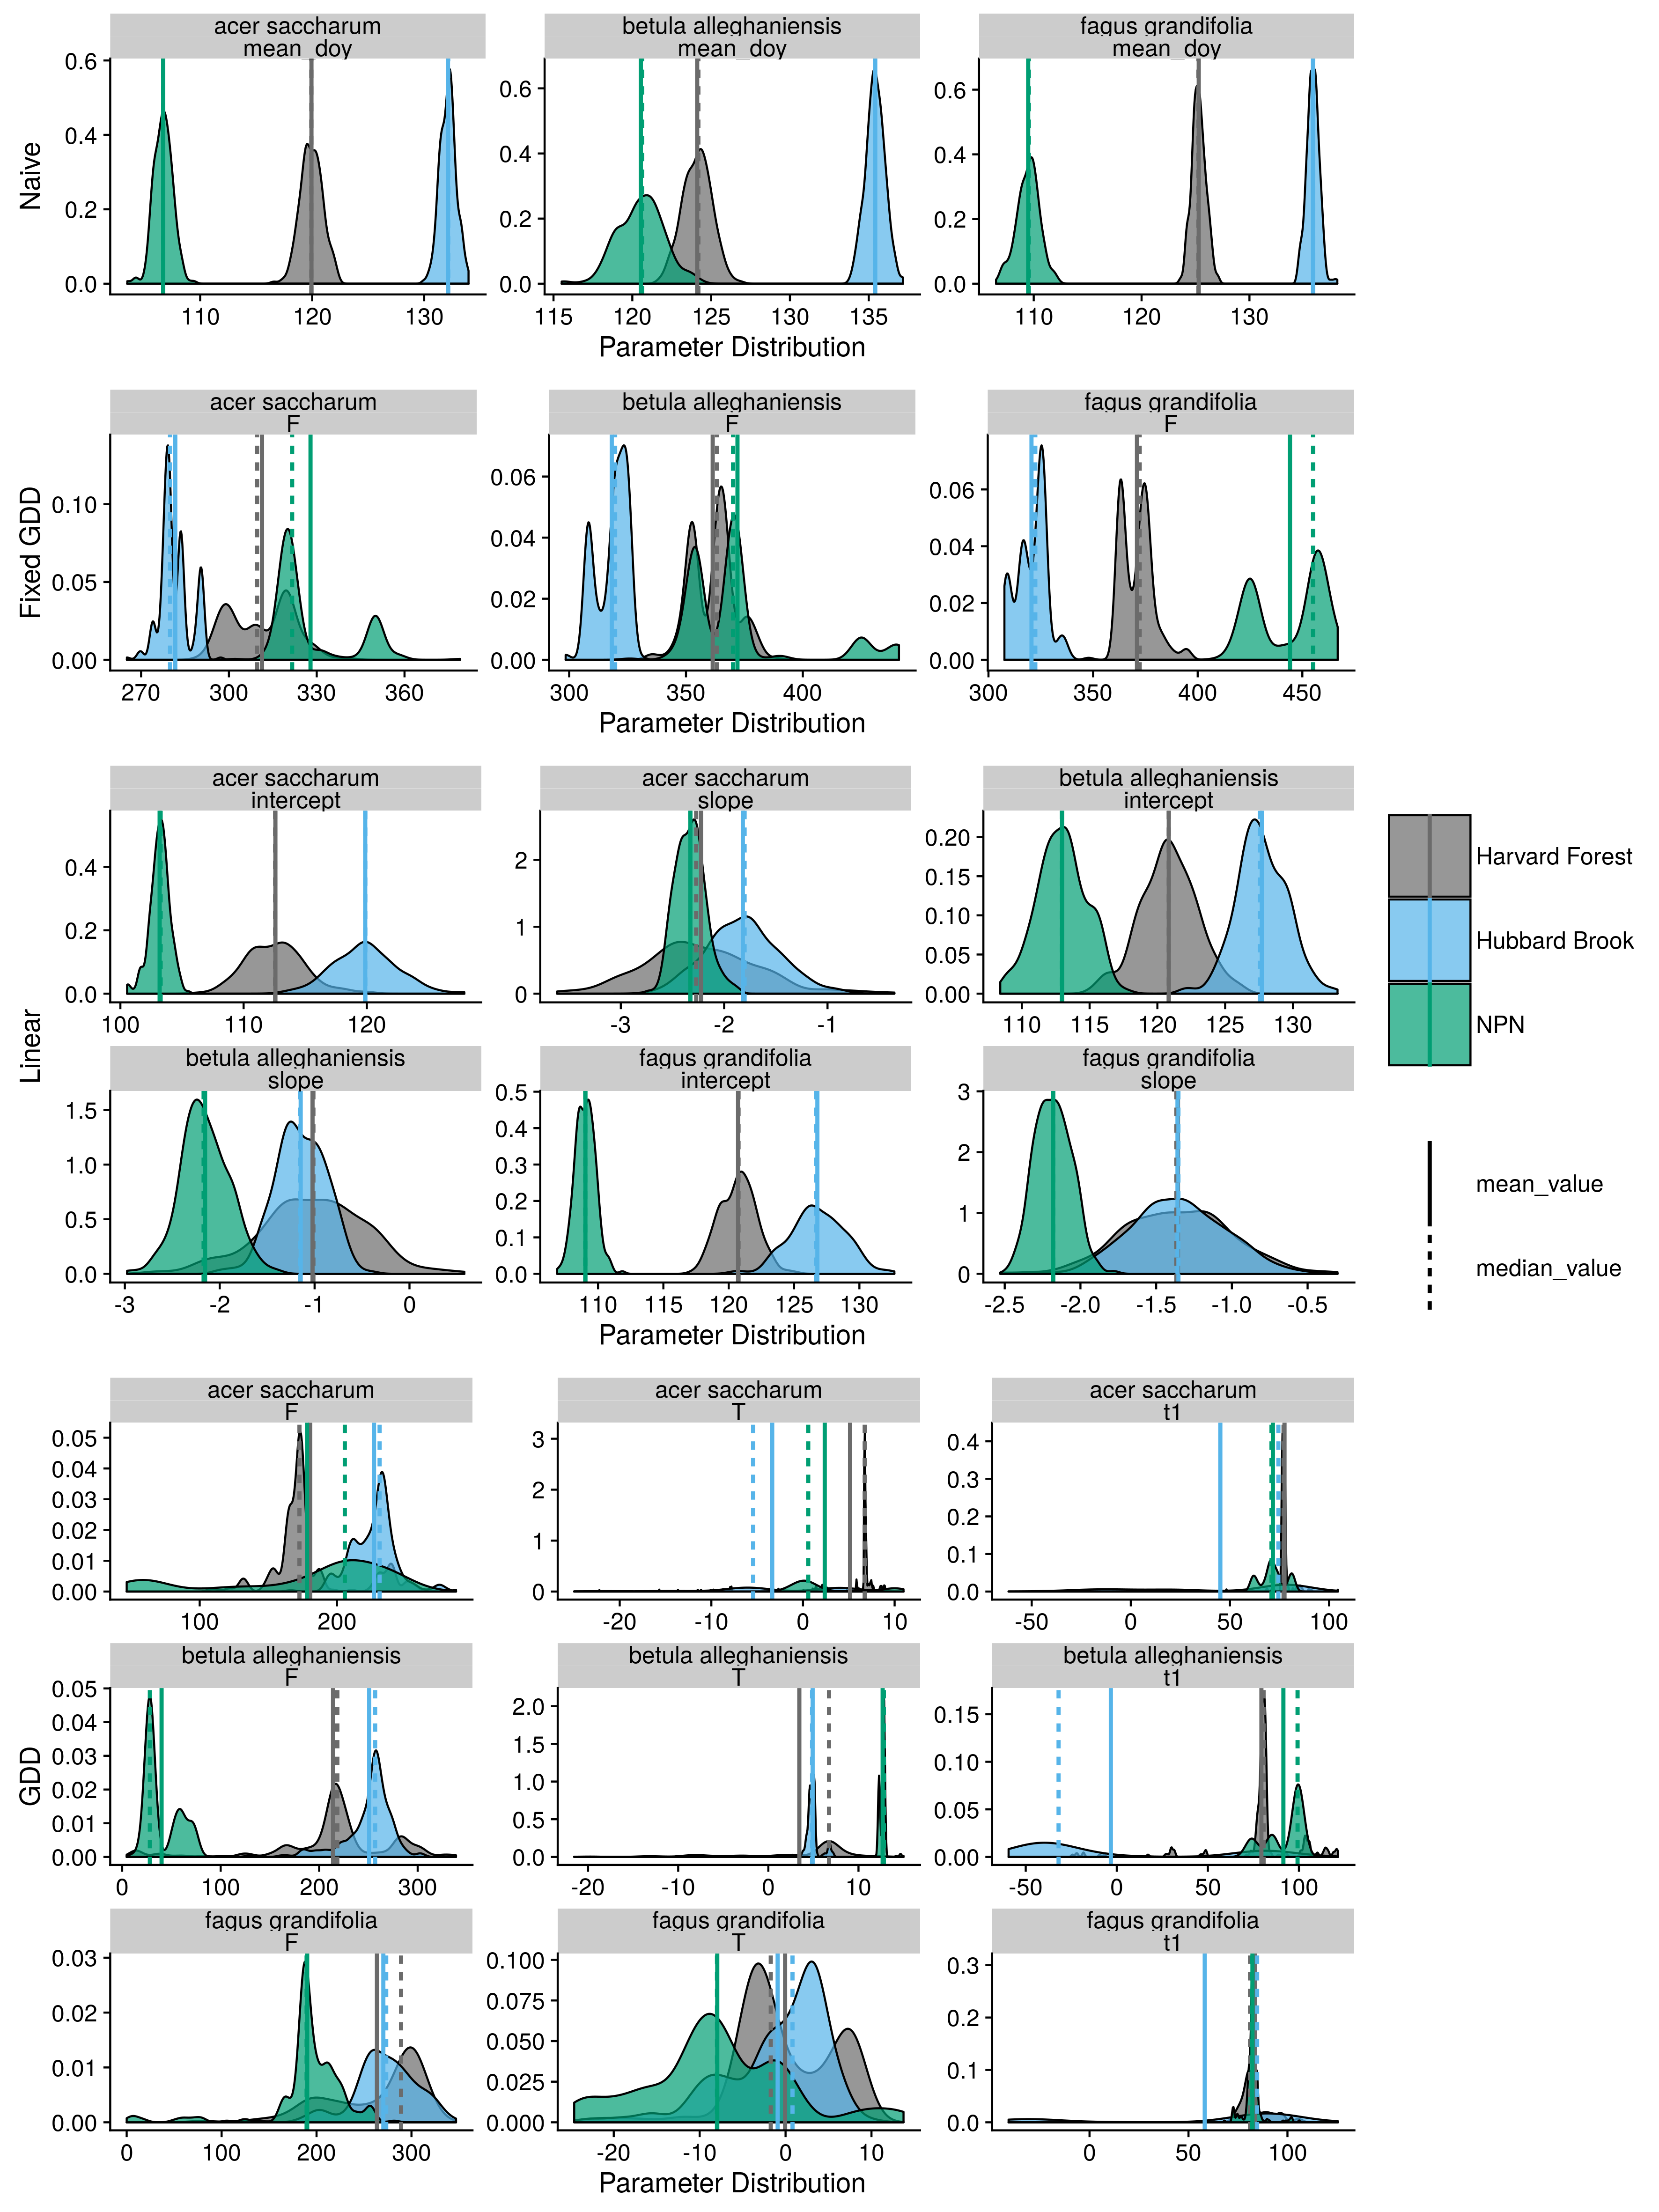
\includegraphics[scale=0.5]{supplement_hubbard_harvard_comparison1.png}
	Figure S4
\end{center}

%%%%%%%%%%%%%%%%%
%% Figure S5
%%%%%%%%%%%%%%%%%
\newpage

\textbf{Figure S5}: As in Figure S4, but for the Alternating and Uniforc models. 

\newpage

\begin{center}
	\centering
		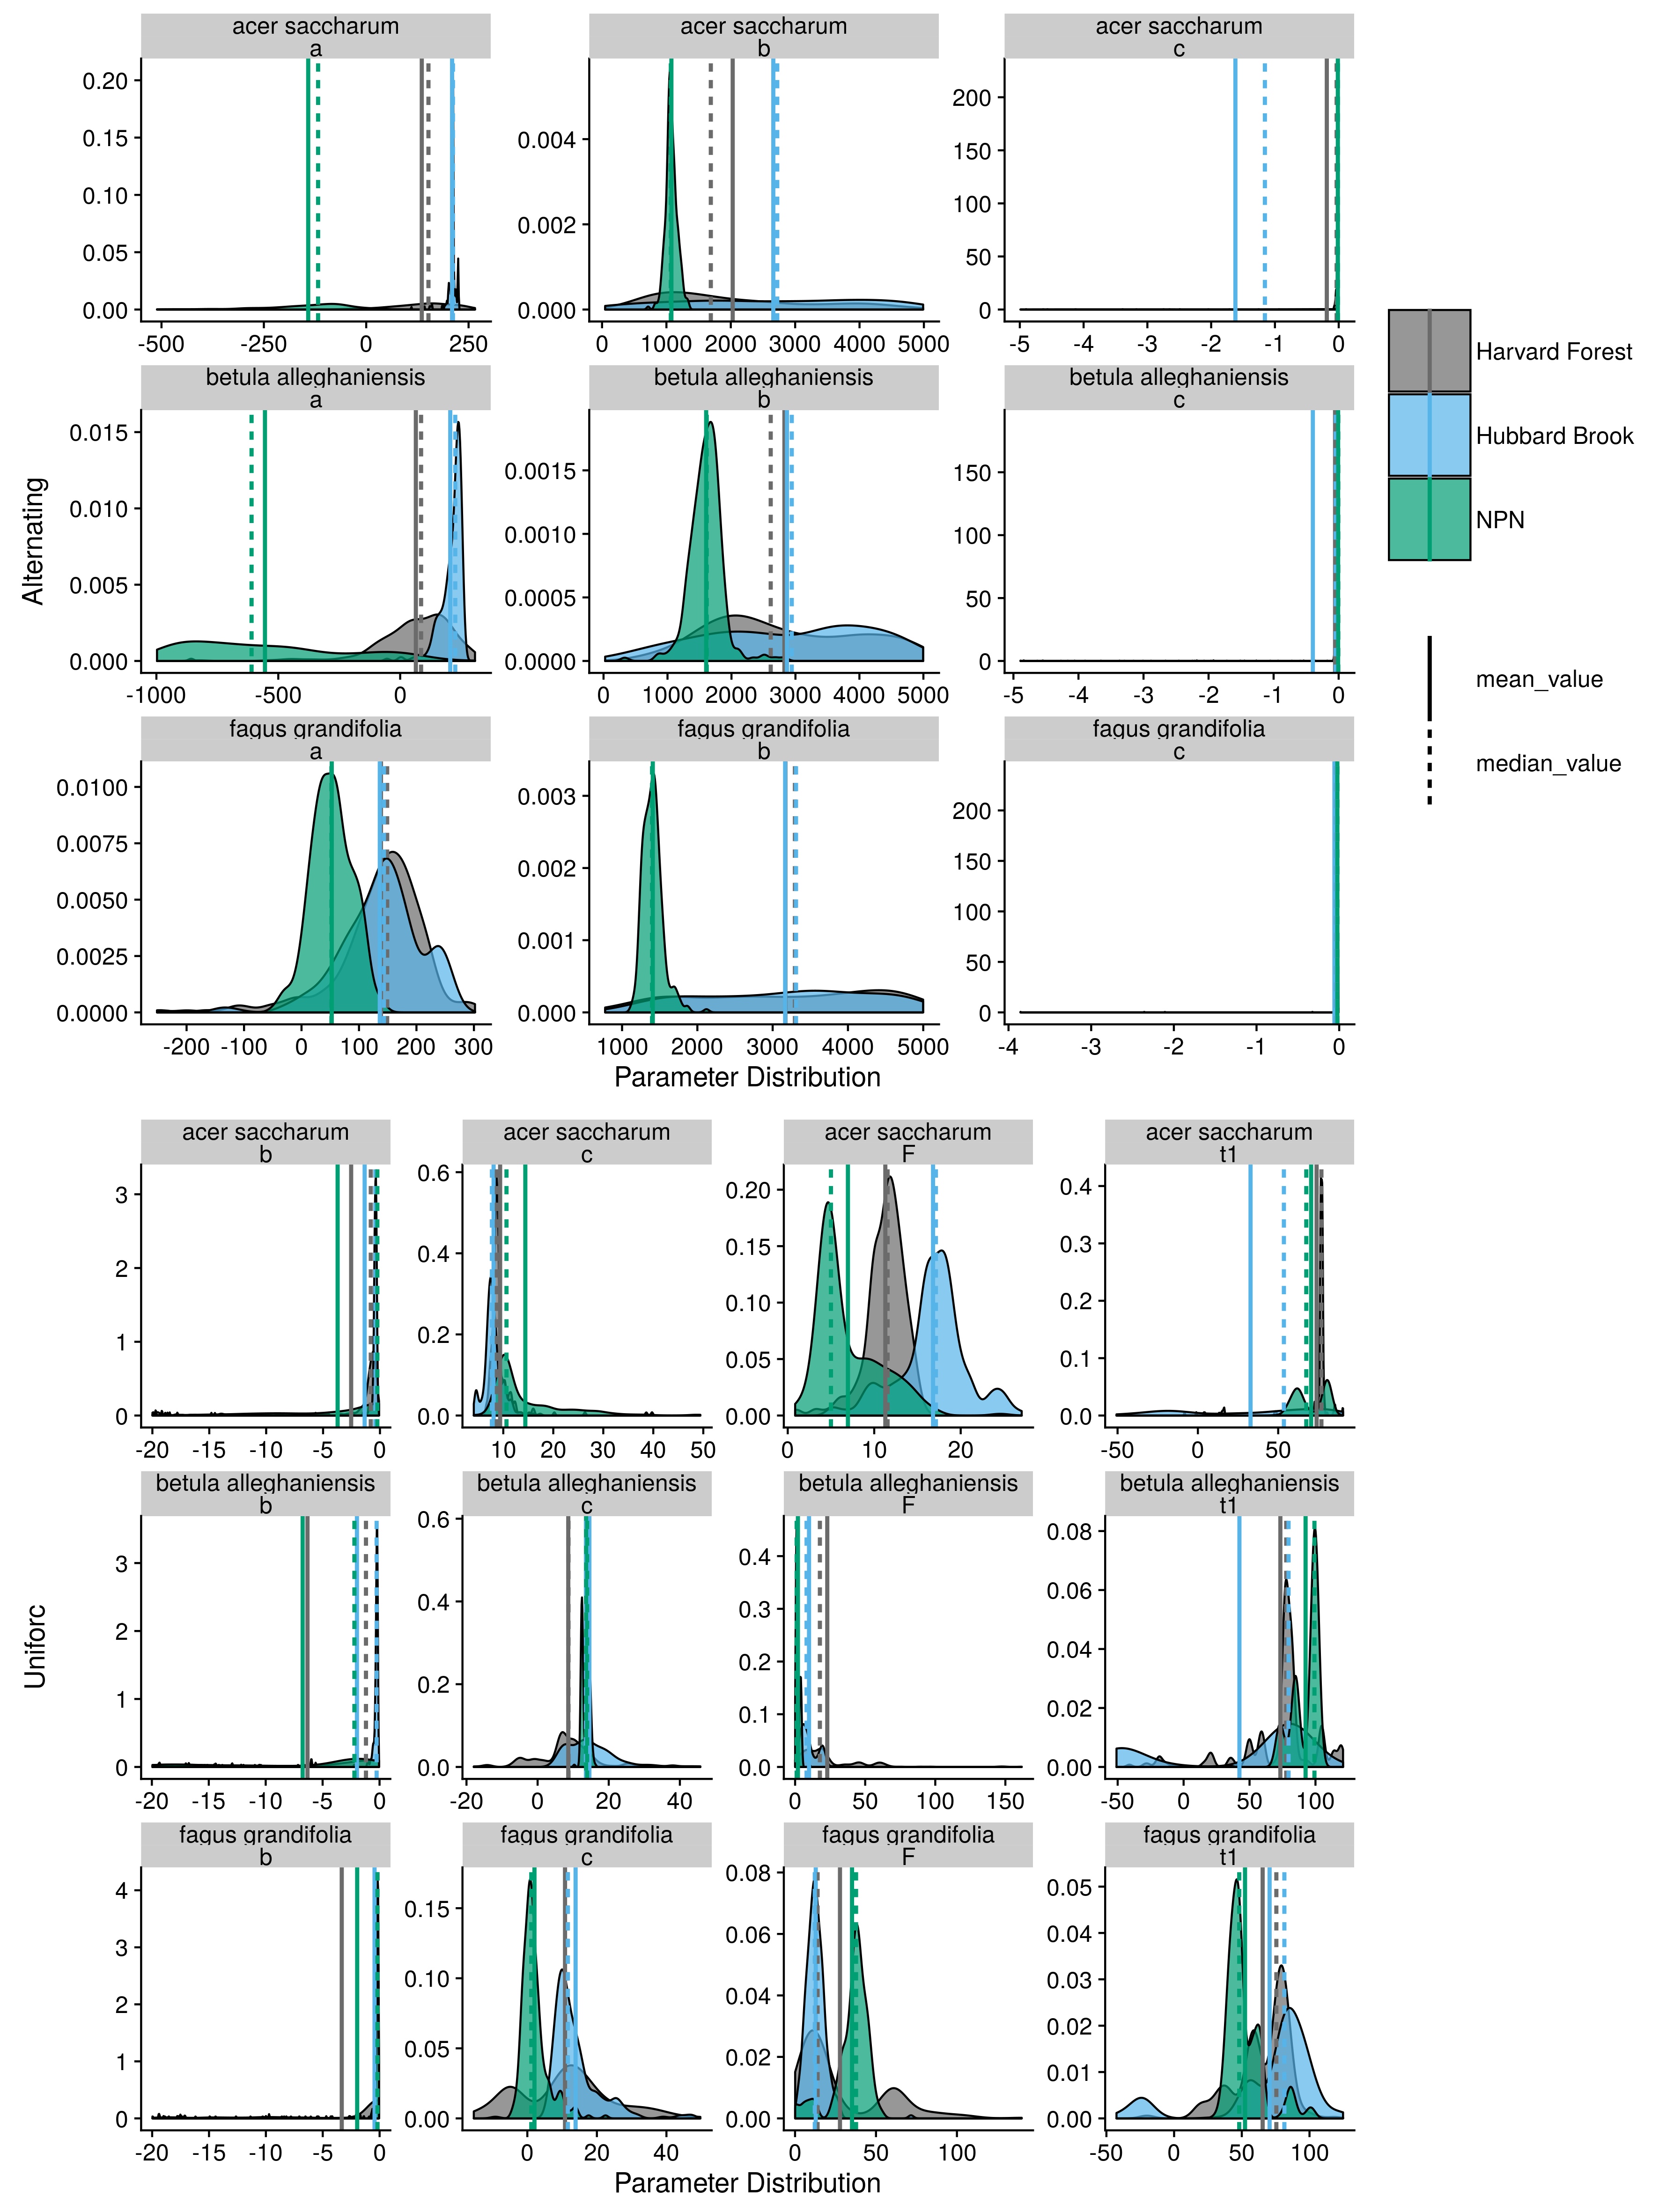
\includegraphics[scale=0.5]{supplement_hubbard_harvard_comparison2.png}
	Figure S5
\end{center}

%%%%%%%%%%%%%%%%%
%% Figure S6
%%%%%%%%%%%%%%%%%
\newpage

\textbf{Figure S6}: As in Figure S4, but for 4 selected species to show the difference in parameter distributions between LTER and USA-NPN derived models. The phenophase for the four species is budburst. These 4 species are representative of the analysis, and for the remaining comparisons the reader is pointed to the script 'analysis/plot\_select\_species\_parameters.R' in the code repository to generate additional figures.

\newpage

\begin{center}
	\centering
		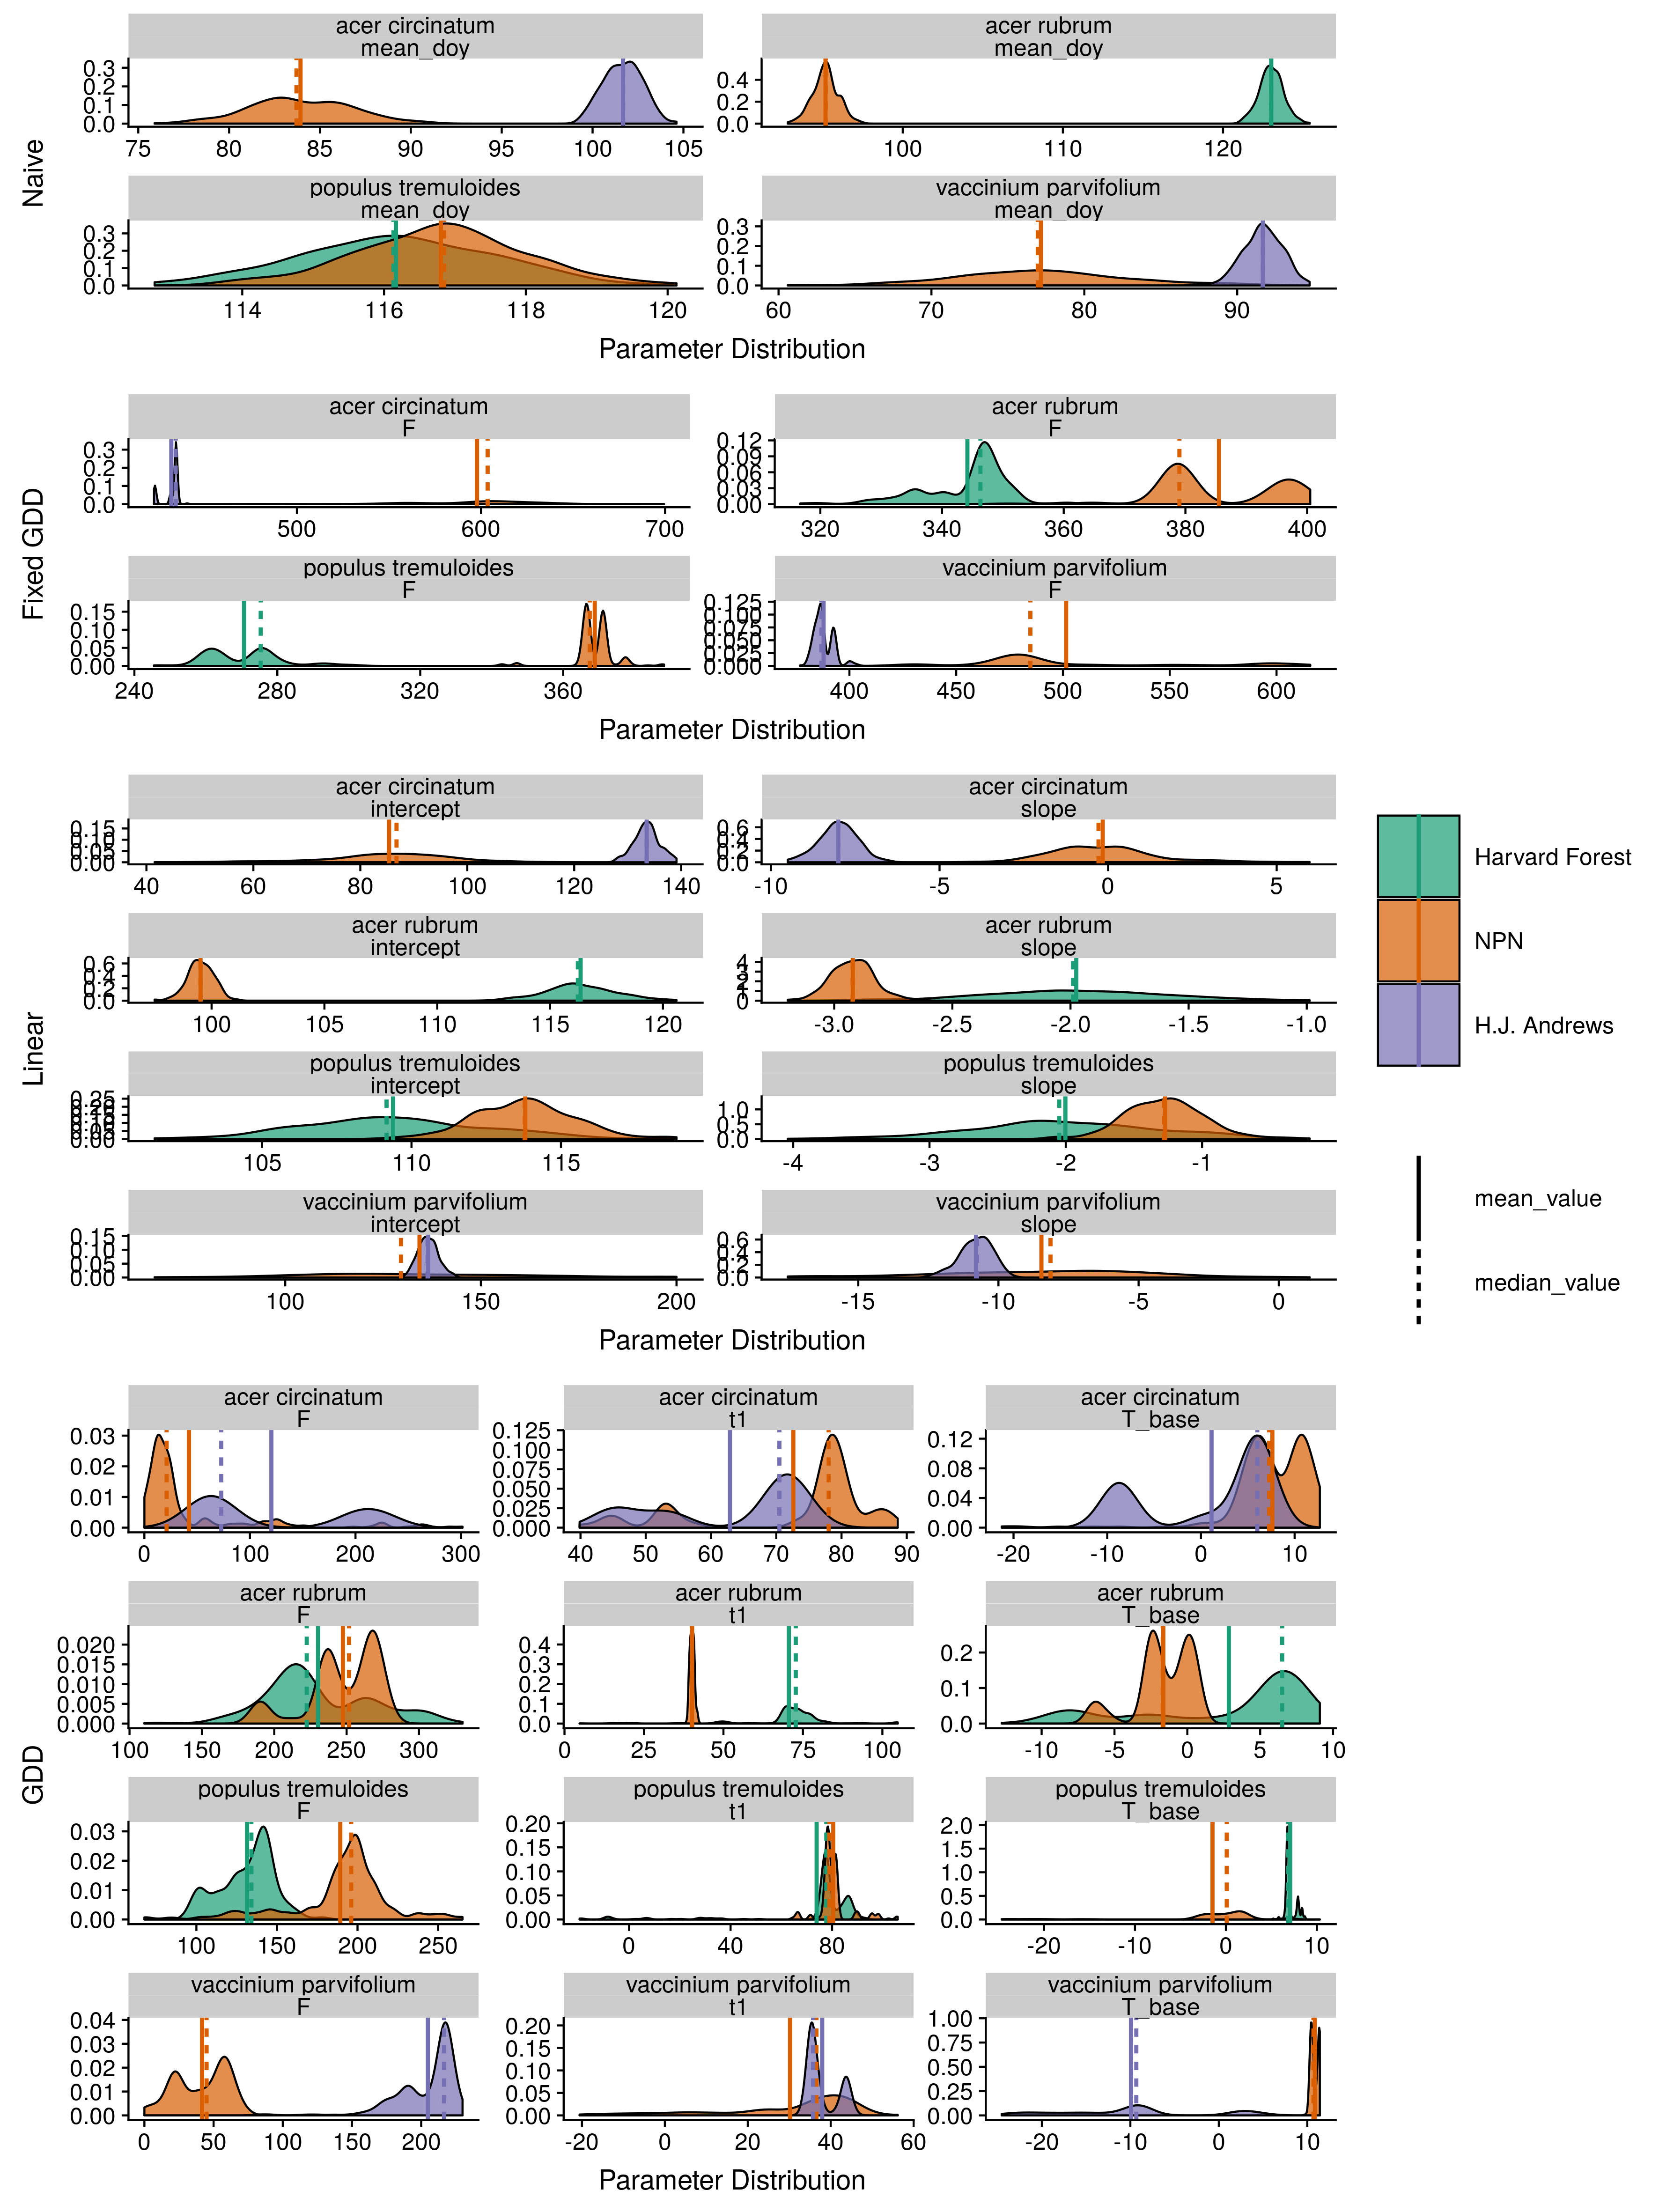
\includegraphics[scale=0.5]{supplement_select_species_param_comparison1.png}
	Figure S6
\end{center}

%%%%%%%%%%%%%%%%%
%% Figure S7
%%%%%%%%%%%%%%%%%
\newpage

\textbf{Figure S7}: As in Figure S6, but for the Alternating and Uniforc models. 

\newpage

\begin{center}
	\centering
		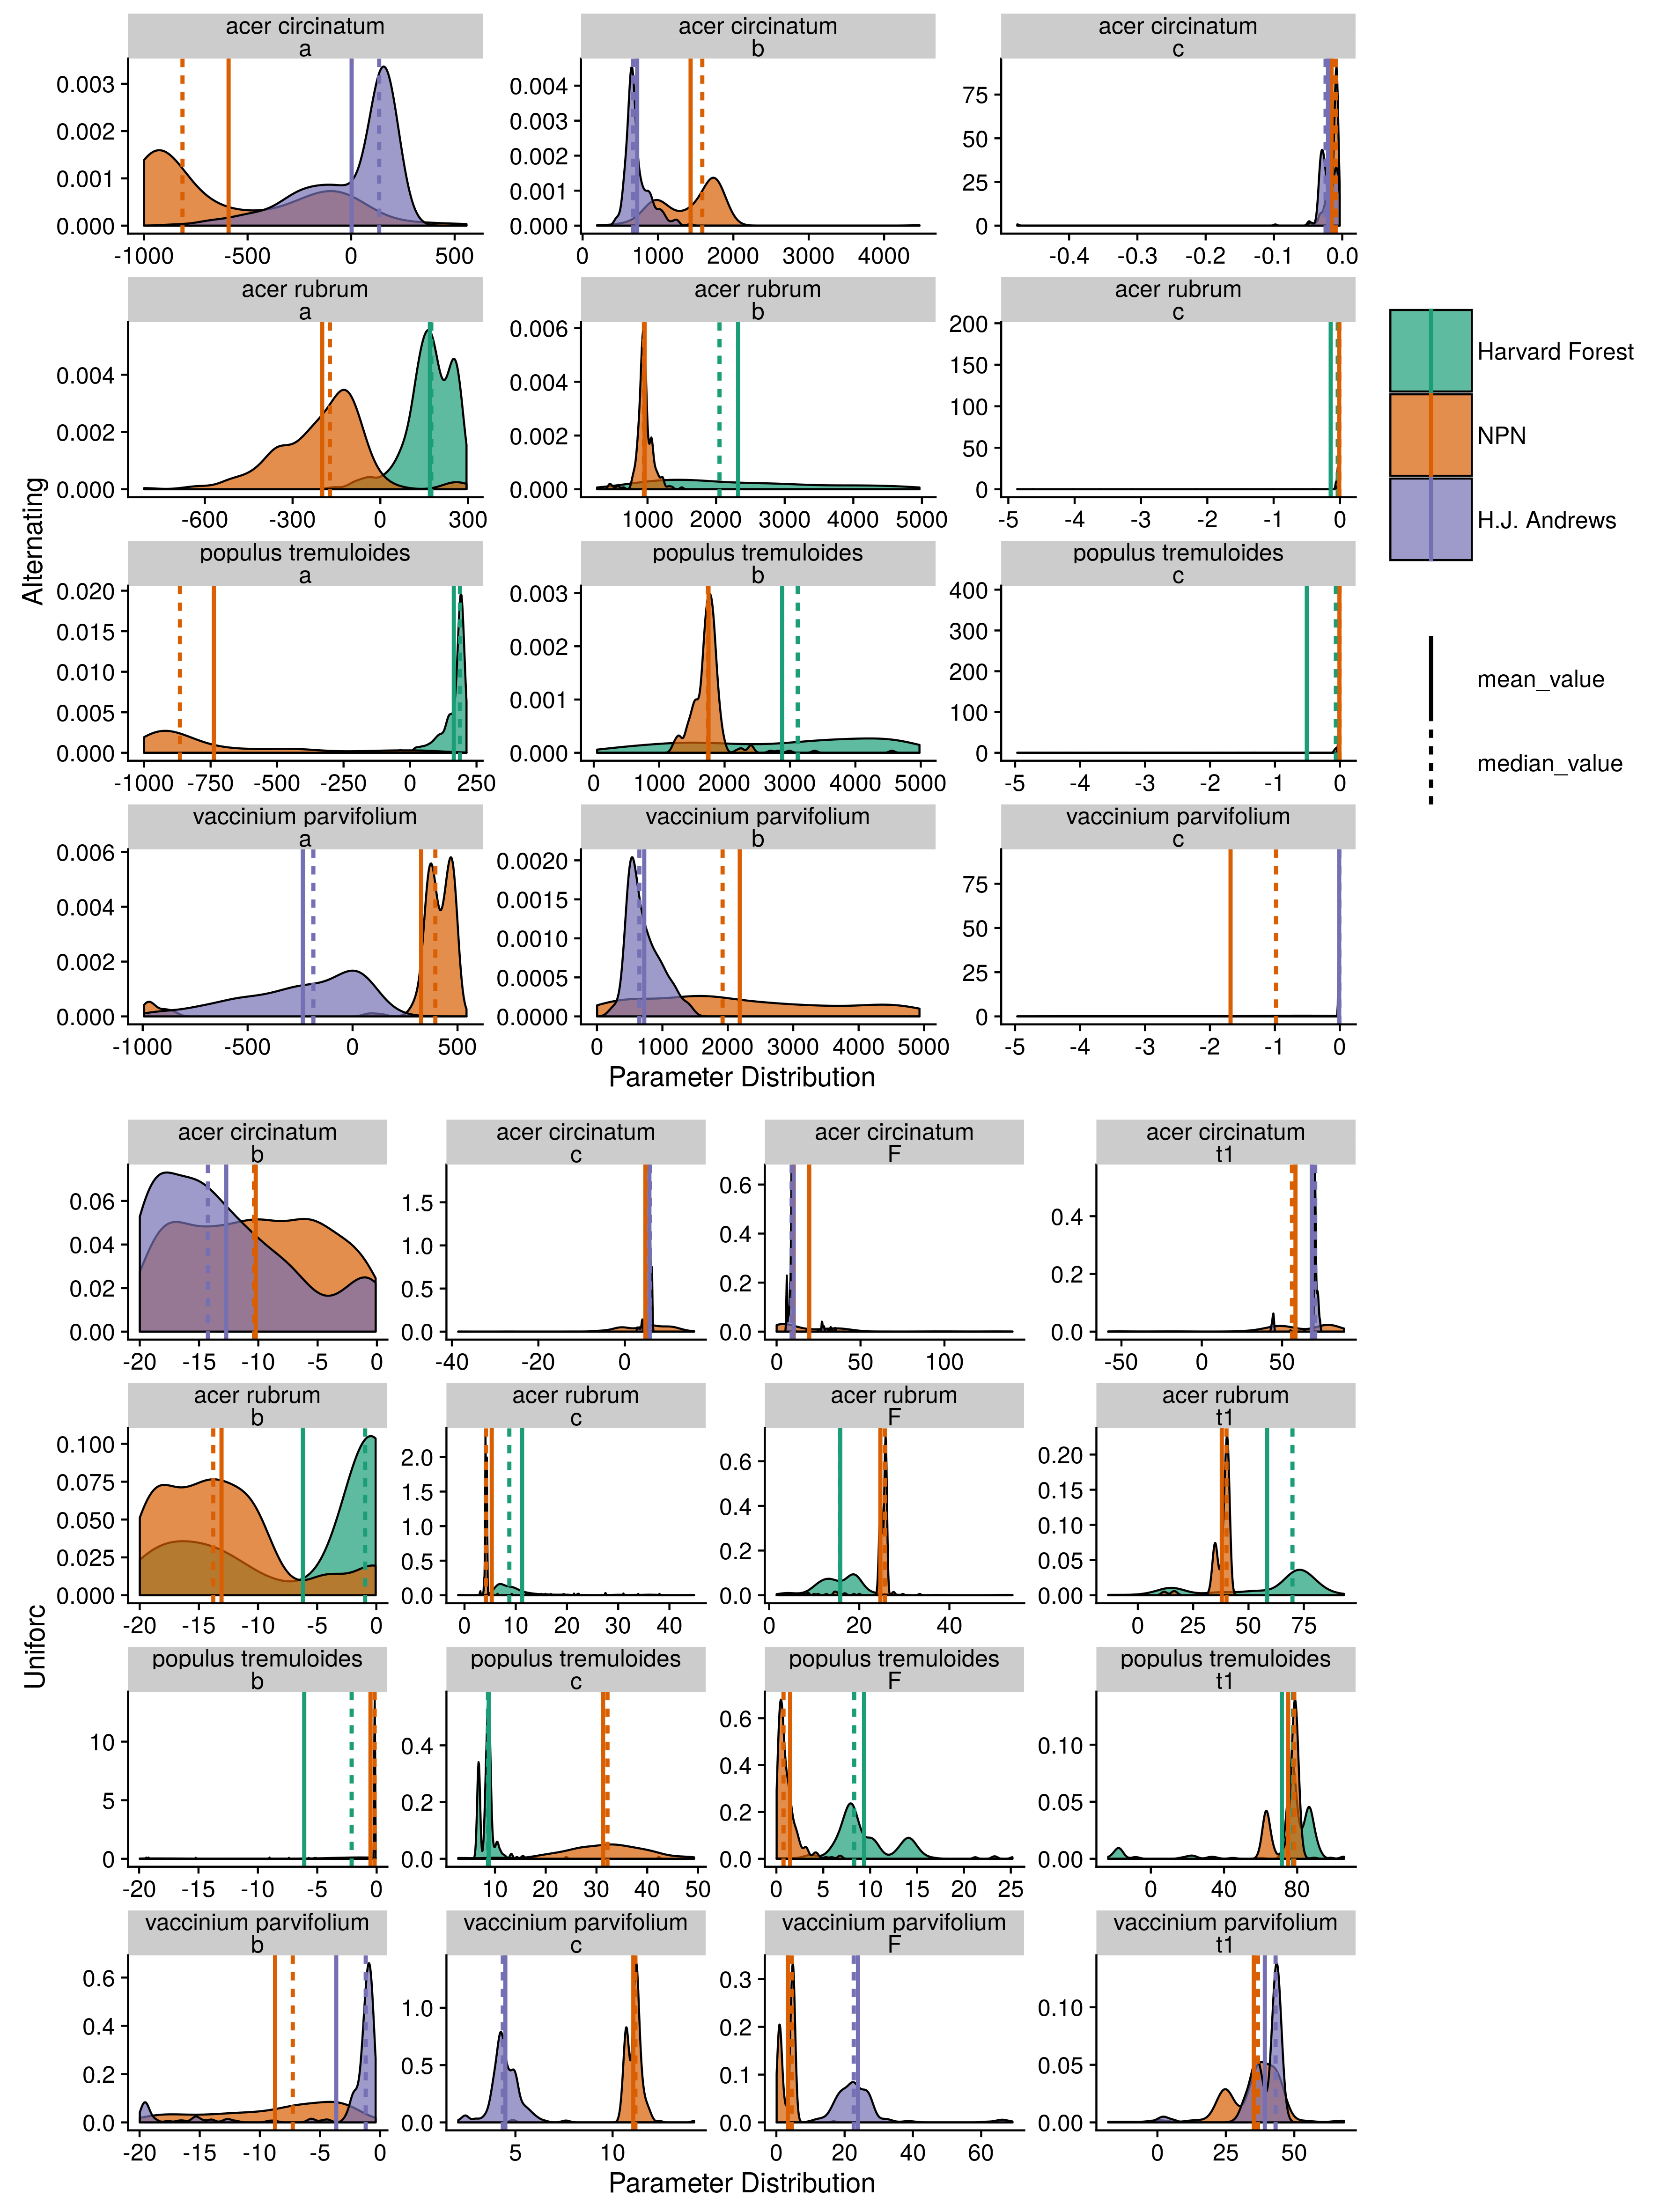
\includegraphics[scale=0.5]{supplement_select_species_param_comparison2.png}
	Figure S7
\end{center}
%%%%%%%%%%%%%%%%%
%% Table S1
%%%%%%%%%%%%%%%%%
\newpage

\textbf{Table S1}: Species used in the analysis along with the sample size from each dataset. The numbers indicate the sample size of the training data and the size of the testing data in parenthesis. 

\newpage

\begin{table}
\tiny
\begin{tabular}{l|r|l|l|l|l|l|l}
\hline
species & phenophase & phenophase\_type & harvard & hjandrews & hubbard & jornada & npn\\
\hline
acer circinatum & 371 & Budburst & - & 266 (66) & - & - & 39 (10)\\
\hline
acer circinatum & 501 & Flowers & - & 116 (29) & - & - & 33 (8)\\
\hline
acer pensylvanicum & 371 & Budburst & 80 (20) & - & - & - & 34 (9)\\
\hline
acer rubrum & 371 & Budburst & 100 (25) & - & - & - & 957 (239)\\
\hline
acer rubrum & 501 & Flowers & 96 (24) & - & - & - & 668 (167)\\
\hline
acer saccharum & 371 & Budburst & 60 (15) & - & 164 (41) & - & 365 (91)\\
\hline
betula alleghaniensis & 371 & Budburst & 60 (15) & - & 178 (44) & - & 133 (33)\\
\hline
betula alleghaniensis & 501 & Flowers & 26 (7) & - & - & - & 64 (16)\\
\hline
betula lenta & 371 & Budburst & 58 (14) & - & - & - & 96 (24)\\
\hline
betula papyrifera & 371 & Budburst & 76 (19) & - & - & - & 96 (26)\\
\hline
betula papyrifera & 501 & Flowers & 18 (5) & - & - & - & 36 (9)\\
\hline
fagus grandifolia & 371 & Budburst & 76 (19) & - & 177 (44) & - & 259 (65)\\
\hline
fraxinus americana & 371 & Budburst & 84 (21) & - & - & - & 90 (23)\\
\hline
fraxinus americana & 501 & Flowers & 22 (6) & - & - & - & 52 (13)\\
\hline
ilex verticillata & 371 & Budburst & 35 (9) & - & - & - & 26 (6)\\
\hline
larrea tridentata & 501 & Flowers & - & - & - & 27 (7) & 118 (30)\\
\hline
nyssa sylvatica & 371 & Budburst & 27 (7) & - & - & - & 63 (16)\\
\hline
pinus strobus & 496 & Budburst & 38 (10) & - & - & - & 77 (19)\\
\hline
populus tremuloides & 371 & Budburst & 38 (10) & - & - & - & 208 (51)\\
\hline
populus tremuloides & 501 & Flowers & 17 (4) & - & - & - & 79 (22)\\
\hline
prosopis glandulosa & 501 & Flowers & - & - & - & 49 (12) & 78 (20)\\
\hline
prunus serotina & 371 & Budburst & 58 (14) & - & - & - & 228 (57)\\
\hline
pseudotsuga menziesii & 480 & Budburst & - & 182 (46) & - & - & 38 (10)\\
\hline
quercus alba & 371 & Budburst & 62 (15) & - & - & - & 174 (43)\\
\hline
quercus rubra & 371 & Budburst & 80 (20) & - & - & - & 242 (60)\\
\hline
quercus rubra & 501 & Flowers & 56 (14) & - & - & - & 127 (32)\\
\hline
quercus velutina & 371 & Budburst & 77 (19) & - & - & - & 72 (18)\\
\hline
rhododendron macrophyllum & 371 & Budburst & - & 84 (21) & - & - & 48 (12)\\
\hline
rhododendron macrophyllum & 501 & Flowers & - & 27 (7) & - & - & 50 (12)\\
\hline
trillium ovatum & 488 & Budburst & - & 222 (55) & - & - & 68 (17)\\
\hline
trillium ovatum & 501 & Flowers & - & 169 (42) & - & - & 60 (15)\\
\hline
vaccinium corymbosum & 371 & Budburst & 38 (10) & - & - & - & 60 (15)\\
\hline
vaccinium corymbosum & 501 & Flowers & 38 (10) & - & - & - & 65 (16)\\
\hline
vaccinium parvifolium & 371 & Budburst & - & 149 (37) & - & - & 25 (6)\\
\hline
vaccinium parvifolium & 501 & Flowers & - & 162 (41) & - & - & 25 (6)\\
\hline
\end{tabular}
\newline
Table S1
\end{table}


\end{document}}
